% This file makes use of sydetex.

% sydetex is free software: you can redistribute it and/or modify
% it under the terms of the GNU General Public License as published by
% the Free Software Foundation, either version 3 of the License, or
% any later version.

% sydetex is distributed in the hope that it will be useful,
% but WITHOUT ANY WARRANTY; without even the implied warranty of
% MERCHANTABILITY or FITNESS FOR A PARTICULAR PURPOSE.  See the
% GNU General Public License for more details.

% You should have received a copy of the GNU General Public License
% along with sydetex.  If not, see <https://www.gnu.org/licenses/>.


\documentclass[12pt]{article}
\usepackage[utf8]{inputenc}
\usepackage{setspace}
\usepackage{CJK}



% THIS IS WHERE ALL THE SYDE STUFF IS
\usepackage{sydestyle}



% Reference tooling package settings - point to where the files are
\graphicspath{figures/}

\addbibresource{references.bib}

\makeglossaries
\newglossaryentry{tits} 
{
    name=tits,
    description={The tits, chickadees, and titmice constitute the Paridae, a large family of small passerine birds which occur mainly in the Northern Hemisphere and Africa. Most were formerly classified in the genus Parus. While commonly referred to as "tits" throughout much of the English-speaking world, these birds are called either "chickadees" (onomatopoeic, derived from their distinctive "chick-a dee dee dee" alarm call)[1] or "titmice" in North America. The name titmouse is recorded from the 14th century, composed of the Old English name for the bird, mase (Proto-Germanic *maison, German Meise), and tit, denoting something small. The former spelling, "titmose", was influenced by mouse in the 16th century.[2] Emigrants to New Zealand presumably identified some of the superficially similar birds of the genus Petroica of the family Petroicidae, the Australian robins, as members of the tit family, giving them the title tomtit, although, in fact, they are not related. }
}

\newglossaryentry{math}
{
    name=mathematics,
    description={Mathematics is what mathematicians do}
}

\newglossaryentry{formula}
{
    name=formula,
    description={A mathematical expression}
}

\newacronym{}{}{}

\newacronym{ocp}{OCP}{over-current protection}

\newacronym{scp}{SCP}{short-circuit protection}

\newacronym{soc}{SoC}{System-On-a-Chip}

\newacronym{cpm}{CPM}{Circuit Protection Module}

\newacronym{api}{API}{Application Programming Interface}

\newacronym{asic}{ASIC}{Application Specific Integrated Circuit}

\newacronym{adc}{ADC}{Analog-to-Digital Converter}


% hyperref is a prissy princess, so we import it here to prevent weirdness with sydetex.sty
\usepackage{hyperref}
\hypersetup{
    bookmarks=false
}



% PERSONAL DETAILS HERE, this sets up title page
\def\reportTitle{Designing a Circuit Protection Sensor Module}
\def\reportDueDate{September 6, 2018}
\def\studentName{Si Teng Liu}
\def\studentNumber{20473965}
\def\company{FireBright Corporation}
\def\lastSemester{3A}



% Form fitting ;)
\title{\reportTitle}
\author{\studentName}
\studentnumber{\studentNumber}
\lastsemester{\lastSemester}
\date{\reportDueDate}
\employer{\company}
\employeraddress{
\begin{CJK}{UTF8}{gbsn}
松江区 莘砖公路 518号 16号楼, Shanghai, China
\end{CJK}
}



% ------------------------------START OF DOCUMENT------------------------------

% You shouldn't need to edit code above this line for the template to work as 
% intended. Just fill in your content and it should work Just Like Magic (TM).

\begin{document}

    
    \startindent
	\makewtrtitle
	\stopindent
	
	
	\begin{singlespace}
        \begin{flushright}
        James Si Teng Liu\\
    	251 Cochrane Terrace\\
	    Milton, ON, Canada, L9T 8C8\\
	    \end{flushright}


		% TODO: CHECK ME IF IT'S STILL FIEGUTH
		Dr. Paul Fieguth, Professor and Department Chair
	
		Systems Design Engineering
	
	    University of Waterloo
	
	    Waterloo, ON
	
	    N2L 3G1\\
	
		Dear Professor Fieguth,
	\end{singlespace}
    
        I have prepared this report, ``\reportTitle" as my 3B Work Report for the Engineering team at \company. This report is the final of three that I must submit as part of my degree requirements, and it has not received any previous academic credit. This report was entirely written by me and has not received any previous academic credit at this or any other institution.\\
    	
    	FireBright designs and manufactures battery charging solutions for electric vehicles. Under the guidance of my manager Chen Jie, I was able to succcessfully produce the electrical specifications and final design of a circuit protection board.\\
    	
    	The purpose of this report is to detail the process and design choices made in the creation of this circuit protection module, as well as major points of learning through the process. \\


	    \noindent
	    Sincerely,\\
	   % 
\includegraphics[scale =0.2]{signature}\\
    	
    	\studentName \\
    	\studentNumber \\
        3B Systems Design Engineering

	% new page at the end of the letter.
	\newpage


	% Abstract
	%\addcontentsline{toc}{section}{Abstract}
	\begin{abstract}
    Fire safety is a critical component of battery technology, on the road to to fulfill this requirement for a new line of products, FireBright has commissioned a new module to address fire safety from both prevention and protection perspectives. This report details with the design and prototyping process of this module. The problem space is familiar territory to the company, with known sensitivity levels to tune the sensors towards. New issues include the demand for a smaller physical size, lower cost, and more robust layout.
	    
    The solution relies mainly on a architectural shift from individual \acrfull{ocp} modules for sub-assemblies to a main \acrshort{ocp} module for a single product. A smaller footprint and more design robustness is borne from making more use of digital logic in place of hardware based detection. The trade-off being made is the speed of activation of the protective measures. Given that a short-circuit protection module is also being planned, this weakness can be shored up for mission-critical circuitry in sub-assemblies, while less critical circuits still enjoy the benefit of a 'centralised' protection system.
	    
    As a result of the design and prototyping.
	\end{abstract}


	% Make a table of contents.
	\phantomsection % this adds the correct hyperref link, if you add custom ToC sections (as per \addcontentsline) USE THIS EXACT ORDERING OF COMMANDS
	\addcontentsline{toc}{section}{Table of Contents}
	\tableofcontents

	% List of figures and tables.
	\phantomsection
	\addcontentsline{toc}{section}{List of Figures}
	\listoffigures
	
	
	\phantomsection
	\addcontentsline{toc}{section}{List of Tables}
	\listoftables
	
	
	\section{Introduction}
    	\pagenumbering{arabic}  % Couldn't figure out how to automate this, but leave this line in to restart page numbers at 1 and with arabic numbers.
	FireBright works in battery technology - specifically lithium-based battery solutions. Their main product is a battery hot-swap system for electric vehicles, for which they design and produce charging stations, battery packs, and vehicle specific framing. 
	
	\paragraph{}
	Due to high energy density and the flammability of the pole materials, fire safety is a critical component of lithium battery maintenance. For the company's new line of products, there is a need for a smaller and more robust \acrfull{cpm} that can be fitted to many different assemblies. As an Engineering Student, designing this module, prototyping, and testing the completed design was the assigned task for my work term.

    \paragraph{A Note on Terminology and Linguistics} - This sproject was done in an electrical engineering dominated environment, as such the terminology used tends toward abbreviated units and electrical shorthand. They will be expanded and explained whenever possible.
  
	\section{Design Space}
	As per the engineering design workflow in FireBright, a great deal of design choices have already been made by the design team for a physical prototype to be green-lit. Specifically, input and output requirements of this module have already been determined, and a microcontroller unit has been selected. The design choices made by myself are entirely in the circuit design, component choice, and board layout to achieve the requirements while following good practice.
	
	\subsection{Pre-Determined Scope\label{sec:pre-determined-scope}}
	At the start of my project, the determined scope consists of a rough architectural outline and two main requirement sets - electrical input/output, and board safety. Electrical I/O being both upper limits to the electrical signal strength (voltage and current) for individual inputs and outputs, and the expected signal profiles. Board safety would consist of absolute maximum ratings for materials, failure modes, and arc distances.
	
    \subsubsection{Architecture\label{sec:architecture}}
    The \acrshort{cpm} is a collection of sensors feeding into a microcontroller, which will communicate the sensor data through a standard transmission protocol used in FireBright's other products. As a system, the module will monitor the sensor data and break a relay switch that controls the main power circuit should sensor readings surpass programmed thresholds. The thresholds have been pre-determined, thus will not be gone into in detail.

    \paragraph{}
    The sensors deemed as required on this module are: two temperature sensors, one smoke sensor, and an AC current sensor. Three components have been chosen ahead of time as required - EFM8BB1 microcontroller, MAX3485 RS-485 transceiver, and a specific current sensing transformer.
    
    \paragraph{}
    Ultimately for each sensor, the signal strength must be scaled to the acceptable input voltage ranges of the microcontroller, and the output must be able to be controlled by the voltage signal generated by the microcontroller as well.

    \paragraph{Physical Response Systems}
    Sensory signals are also part of the requirement of the system, with controllable LED and buzzer components marked as required.

    \subsection{Input and Output} 
    There are two main types of electrical communication between the various system components - signal and power. The power electric behaviour is outlined as a single power supply source, followed by power modulation units that filter and deliver steady power to the components. The specifics would be determined through the design process.

    \paragraph{}
    The signal behaviour were also delivered as a general outline of component intercommunication \footnote{i.e. - Must have communication from sensor to MCU, MCU to transceiver, and so on.}. The final signal profiles were reached through design, testing, and analysis.

    \paragraph{}
    Ultimately, input and output signal levels and limits are left as an excercise for the student to develop, with reference to the specified components - both explicitly named (MCU and Transceiver), and general (sensors needed, relay).
     

    \subsection{Power considerations}
    As the module is going to be a safety mechanism, it is intended to stay powered at all times, thus power draw is specifically budgeted at less than 1 watt on average.
    

	
  \subsection{Developing Criteria}
  Given the scope and requirements set out at the start of the project, a number of criteria can be extracted from the pre-determined components. The specifcations of the MCU will determine the required output levels of all the sensors, and the MCU controlled devices must necessarily respond to the signals that it is capable of delivering.

  To that end, a connection diagram was made to 

  \begin{table}[]
    \caption{A connection chart detailing the input output connections (with directionality)}
    \label{tab:connect_diag}
    \begin{tabular}{rccccccccccc}
      Transmitter \textbackslash Receiver & EFM8BB & MAX3485 & DT-CT & smoke & led & sound & relay & temp0 & temp1 & ldo3v3 & ldo5v0 \\
      EFM8BB                              & -      & 1       &       &       & 1   & 1     & 1     &       &       &        &        \\
      MAX3485                             & 1      & -       &       &       &     &       &       &       &       &        &        \\
      DT-CT                               & *      &         & -     &       &     &       &       &       &       &        &        \\
      smoke                               & 2      &         &       & -     &     &       &       &       &       &        &        \\
      temp1                               & *      &         &       &       &     &       &       & -     &       &        &        \\
      temp1                               & *      &         &       &       &     &       &       &       & -     &        &        \\
      ldo3v3                              & 1      & 1       &       &       &     &       &       & 1     & 1     & -      &        \\
      ldo5v0                              &        &         &       & 2     &     & 2     &       &       &       & 2      & -     
    \end{tabular}
  \end{table}

  \begin{figure}[]
    \centering
    \caption{Connection chart detailing the input and output relationships between the components. The connections go from the components in the left column to the components in the top row.}
    \label{fig:connect-diag}
    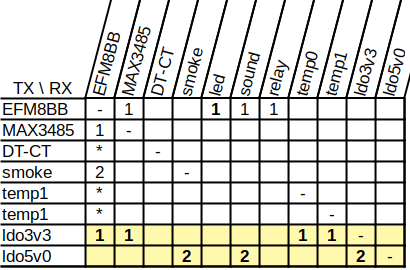
\includegraphics{connection-chart.png}
  \end{figure}
	
  The operating voltage level of the EFM8BB1 family is 3.3V, thus the sensor circuitry must conform to this level. There eventually arose a need for a separate 5V signal level due to the smoke sensor's digital circuit, resolving this will be touched upon in section \ref{sec:devel-electr-design}.

  \section{Component Based Criteria}

  From the datasheet of the EFM8BB1\cite{silabs:efm8bb1}, 

	\section{Understanding Limitations}
	\subsection{Resources}
  \subsubsection{Accuracy of Measurement Tools}
	\subsection{Tooling Available}
	
	
	
	\section{Developing Electrical Design\label{sec:devel-electr-design}} 
	\subsection{Power}
  

  - Relay uses raw input - set input to sane value
  - speaker power is switched by the MCU, power delivered by the LDO
	
	\section{Developing Mechanical Specifications}
	
	
	\section{Component Selection}
	
	\section{Final Electrical Design}
	
	
    \printglossaries
    
    \phantomsection
    \printbibliography[heading=bibintoc]
	

\end{document}


